\chapter{Electrostatic equation -- Capacitance of two balls}

\modinfo{Directory}{CapacitanceOfTwoBalls}
\modinfo{Solvers}{\Idx{StatElecSolver}}
\modinfo{Tools}{\Idx{netgen},\Idx{ElmerGUI}}
\modinfo{Dimensions}{3D, Steady-state}
\modinfo{Author}{Peter R{\aa}back}



\subsection*{Case definition}

This case presents the solution of the capacitance of perfectly conducting balls in free space. 
A voltage difference between the balls results to electric charge being introduced to the system. The balls have 
also self-capacitance that comes from the voltage difference with the far field. Therefore a symmetric capacitance matrix
with of size $2\times2$ needs to be solved.
The capacitances may be computed from two different voltage configurations.
For both the electrostatic equation is solved automatically. 

The problem does not have an analytical solution in a closed form. 
However, the cross-capacitance between the balls may be approximated from the series solution~\cite[Ch.~A.3]{wasshuber97}:
\begin{equation}
C_{12} = 4 \pi \varepsilon \frac{a^2}{d}\left ( 1 + \frac{a^2}{d^2-2a^2} + \frac{a^4}{d^4-4d^2a^2 + 3a^4}+ \ldots \right )
\end{equation}
and the self-capacitance from 
\begin{equation}
C_{10} = C_{20} = 4 \pi \varepsilon a \left ( 1 - \frac{a}{d} + \frac{a^2}{d^2-a^2} - \frac{a^3}{d^3-2da^2}+ \ldots \right )
\end{equation}
Let's mark $\tilde{C} = C / \varepsilon$. In this case $\tilde{C}_{12} \approx 1.191$ and $\tilde{C}_{10} \approx 5.019$.
Unfortunately the error bounds are not given.

In this particular case 
the balls are assumed to have a radius of $a=0.5$ and they are placed at distance $d=2$ apart from 
each other (measured from the ball origins). 


\subsection*{Meshing with Netgen (Optional)}

If you have Netgen installed and running, then you can generate the mesh before starting ElmerGUI, following the below instructions.  

If you don't have Netgen available, don't worry, an Elmer mesh has been provided in the `CapacitanceOfTwoBalls'  subfolder under `tutorials-GUI-files'.  Just load the ElmerGUI project in that subfolder, and it will load the mesh for you.  After loading the mesh, skip ahead to the next section, `Solution Procedure'.

If you have Netgen installed, then meshing is performed with the graphical user interface of Netgen. Netgen creates tetrahedral quality meshes and provides a native output for Elmer.
At the time of writing this tutorial the quadratic elements had some problems with numbering 
but these should not affect the linear elements.

The file is given as netgen geometry format in file \texttt{TwoBallsInBall.geo}. The geometry definition includes the 
two smaller balls inside a bigger ball. Ultimately the bigger ball would be infinitely large. As this is impossible 
here we choose a modest radius of 5. The larger this value, the better the far-field approximation of the 
electrostatic solution is.

The content of the file is given below:
\ttbegin
#
# a large ball with two smaller balls cut off
#
algebraic3d
solid smallballs = sphere (-1.0, 0.0, 0.0; 0.5)
           or sphere (1.0, 0.0, 0.0; 0.5);
solid bigball = sphere (0.0, 0.0, 0.0; 5.0);
solid rest = bigball and not smallballs;
tlo rest -col=[0,0,1] -transparent;
\ttend

Open the file and apply the default meshing. In this example two consecutive uniform refinements were performed 
(choose \texttt{Refine Uniform} under \texttt{Refinemenent}) so that the 
final mesh consisted of 41\,693 nodes and 238\,976 linear tetrahedrons. 

To save the mesh first choose under \texttt{File} the \texttt{Export Filetype} to be \texttt{Elmer}. Then choose
\texttt{Export Mesh} and save the mesh into a suitable directory to be opened
by ElmerGUI. 

\begin{figure}[h]
\centering
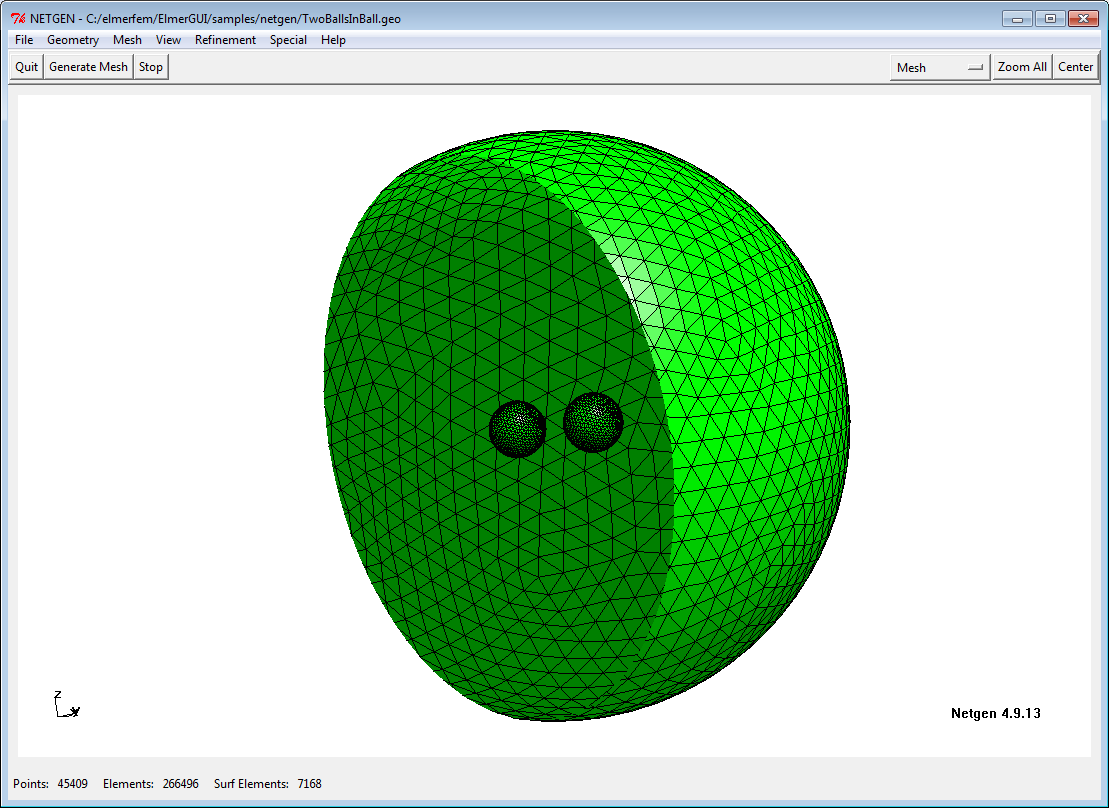
\includegraphics[width=140mm]{netgen_capture}
\caption{Surface mesh for the two inner balls as seen in Netgen}\label{fg:ballsnetgen}
\end{figure}  

The order of the mesh using nodal elements 
may be increased by \texttt{ElmerGrid}. Assuming the mesh would reside in directory \texttt{meshlin}
a mesh consisting of quadratic elements may be performed with the following command:
\ttbegin
ElmerGrid 2 2 meshlin -increase -out meshquad
\ttend
This will maintain the number of elements but the number of nodes will, in this case, increase to 359\,009. 


\subsection*{Solution procedure}

The definitions for the electrostatic equation may not have been loaded into ElmerGUI by default. If this is the case 
one needs to load these before starting the simulations.
\ttbegin
File 
  Definitions
    Append -> electrostatics.xml
\ttend
The additional definitions should reside in the directory \texttt{edf-extra} within the distribution.
Moving the desired \texttt{xml} files to the \texttt{edf}-directory enables automatic loading of the 
definitions at start-up. By inspecting the definitions in the \texttt{Elmer Definitions File editor} one
may inspect that the new definitions were really appended. 


The mesh is already created, load it from the directory that was created above.
\ttbegin
File 
  Load Mesh -> mesh
\ttend

\begin{figure}[h]
\centering
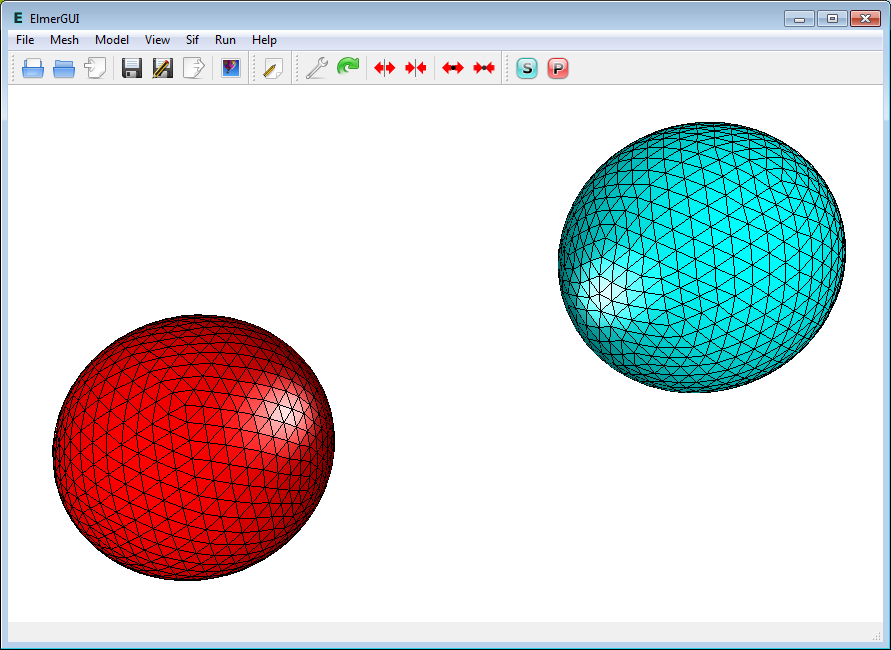
\includegraphics[width=140mm]{ElmerGUI_capture}
\caption{The mesh with one highlighted ball as seen in ElmerGUI}\label{fg:ballselmergui}
\end{figure}  

The display in ElmerGUI upon loading the mesh will show the outside of the large ball.  
To view the inner two smaller balls, double click on the outside of the large ball, then 
click on `Hide/show selected'.

\ttbegin
View 
  Hide/show selected   Ctrl+H
\ttend


After we have the mesh we start to go through the Model menu from the top to bottom. 
In the Setup we choose things related to the whole simulation such as file names, 
time stepping, constants etc.
The steady-state simulation is carried out in 3-dimensional Cartesian
coordinates. For convenience we also set the permittivity of vacuum $\varepsilon_0$ equal to one.
This makes it easier to compare the results to the analytical expressions. 
\ttbegin
Model
  Setup 
    Simulation Type = Steady state
    Vacuum Permittivity = 1.0
\ttend
In the equation section we choose the relevant equations and parameters related to their solution. 
In this case we'll have only the electrostatics solver. 

When defining Equations and Materials it is possible to assign to the bodies immediately, or to use mouse
selection to assign them later. In this case we have just one body and therefore its easier to assign 
the Equation and Material to it directly.

In the solver specific options we want to activate some flags that are needed to invoke the 
computation of derived fields. 
For the linear system solvers we are happy to use the defaults. One may however, try out different
preconditioners (ILU1,\ldots) or direct Umfpack solver, for example.
\ttbegin
Model
  Equation
    Name = Electrostatics
    Apply to Bodies = 1
    Electrostatics
      Active = on
      Edit Solver Settings
        Solver specific options
          Calculate Capacitance Matrix = True
          Calculate Electric Field = True
          Calculate Electric Energy = True
    Add 
    OK
\ttend        
The Material section includes all the material parameters.
In this case we only have the relative permittivity $\varepsilon_r$ which we set to one.
\ttbegin
Model
  Material
    Name = Ideal
    Electrostatics
      Relative Permittivity = 1.0
    Apply to Bodies = 1 2
    Add
    OK
\ttend

We have two boundary conditions for the potential at the ground and at the capacitor. For other boundaries
the do-nothing boundary results to zero flux over the boundary.
\ttbegin
Model
  BoundaryCondition
    Name = Farfield
    Electrostatics
      Electric Infinity BC = True
    Add
    New

    Name = CapBody1
    Electrostatics
      Capacitance Body = 1
    Add
    New

    Name = CapBody2
    Electrostatics
      Capacitance Body = 2
    Add
\ttend   

The conditions may also be assigned to boundaries in the Boundary condition menu, or 
by clicking with the mouse. Here we use the latter approach as that spares us of the 
need to know the indexes of each boundary.
\ttbegin
Model
  Set boundary properties
    Choose Outer sphere -> set boundary condition Farfield
    Choose one inner sphere -> set boundary condition CapBody1
    Choose the other inner sphere -> set boundary condition CapBody2
\ttend

For the execution 
ElmerSolver needs the mesh files and the command file. We have now basically defined
all the information for ElmerGUI to write the command file. After writing it we may also visually 
inspect the command file.
\ttbegin
Sif 
  Generate
  Edit -> look how your command file came out  
\ttend

Before we can execute the solver we should save the files in a directory. The project includes
all the files needed to restart the case.
\ttbegin
File 
  Save Project
\ttend

After we have successfully saved the files we may start the solver
\ttbegin
Run
  Start solver
\ttend
A convergence view automatically pops up showing relative changes of each iteration.
The equation is fully linear and hence only two iterations are needed -- the second 
one just ensures that convergence of the non-linear level was really obtained. 
The norm of the solution should be?

When the solution has finished we may start the postprocessor to view some results.
\ttbegin
Run
  Start ParaView
\ttend


\subsection*{Results}

The essential result of this case are the values of the capacitance matrix.
In this case $\tilde{C}_{12} \approx 1.691$ and $\tilde{C}_{10} \approx 5.019$.
For linear elements the obtained figures are 1.6983, 5.0793 and 5.0812, 
for quadratic Lagrange elements 1.6641, 5.0340 and 5.0340, respectively, and
finally for quadratic p-elements 1.6856, 4.9863 and 4.9884. 

The values are rather satisfactory with a difference less than 2\% from the series approximation.


\begin{figure}[h]
\centering
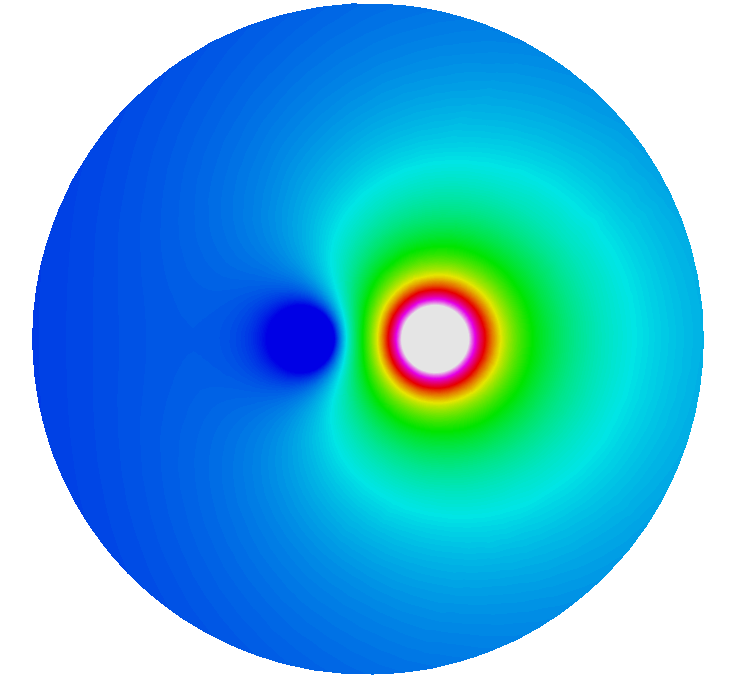
\includegraphics[width=120 mm]{ElmerPost_capture2}
\caption{The electrostatic potential on the clipping plane. This is the latter of the two symmetric configurations where the
unit voltage is applied to one ball and zero voltage to the other, respectively.}\label{fg:ballspost}
\end{figure}  

Note that the derived fields in the StatElecSolver are computed 
by averaging the fields over elements -- not using the 
Galerkin method which would provide optimal accuracy. To get optimal accuracy, use 
\texttt{FluxSolver}, for example


\hfill

\bibliography{tutorialsbib}
\bibliographystyle{plain}
